% @Author: Your name
% @Date:   2024-04-20 21:21:00
% @Last Modified by:   Your name
% @Last Modified time: 2024-04-30 23:52:00
% sectionis/method.tex

 \section{Mathematical Formulation and Problem Statement}\label{sec:formula}
\subsection{Mathematical Formulation of Co-clustering}
Co-clustering is a method designed to simultaneously group a set of rows and columns in a data matrix $\mathbf{A} \in \mathbb{R}^{M \times N}$, where $M$ denotes the number of features or variables and $N$ denotes the number of samples or objects. Each element $a_{ij}$ in the matrix at the $(i, j)$-th position represents the relationship or measurement between the $i$-th feature and the $j$-th object. The primary goal of co-clustering is to identify subsets of rows ($I$) and columns ($J$) into homogenous submatrices, $\mathbf{A}_{I, J}$, that exhibit distinctive patterns or uniform characteristics, thus forming coherent co-clusters. The objective is to partition $\mathbf{A}$ into $k$ row clusters and $d$ column clusters, resulting in $k \times d$ distinct co-clusters.

When rows and columns are optimally reordered, $\mathbf{A}$ can be visualized as a block-diagonal matrix, where each block represents a co-cluster with higher similarity within than between blocks. We define the row and column label sets as \( u \in \{1,\dots,k\}^M \) and \( v \in \{1,\dots,d\}^N \), respectively. Indicator matrices \( R \in \mathbb{R}^{M \times k} \) and \( C \in \mathbb{R}^{N \times d} \) are used to assign rows and columns to clusters, with the constraints \( \sum_k R_{i,k} = 1 \) and \( \sum_d C_{j,d} = 1 \), ensuring each row and column is assigned to exactly one cluster.
 
\subsection{Problem Statement}
This paper aims to develop a method that efficiently and accurately identifies co-clusters $\mathbf{A}_{I, J}$ within a matrix $\mathbf{A}$ representing large datasets. These co-clusters should exhibit specific structural patterns such as uniformity across elements, consistency along rows or columns, or patterns demonstrating additive or multiplicative coherence. Properly identifying and categorizing these patterns is crucial for understanding the complex data structures inherent in large datasets. This method is intended to improve the detection capabilities of co-clustering, enhancing both the efficiency and precision necessary for handling large-scale data challenges.


\section{The Scalable Co-clustering Method}
\label{sec:method}
\subsection{Overview}

% insert workflow.png here
\begin{figure*}[htbp]
    \centering
    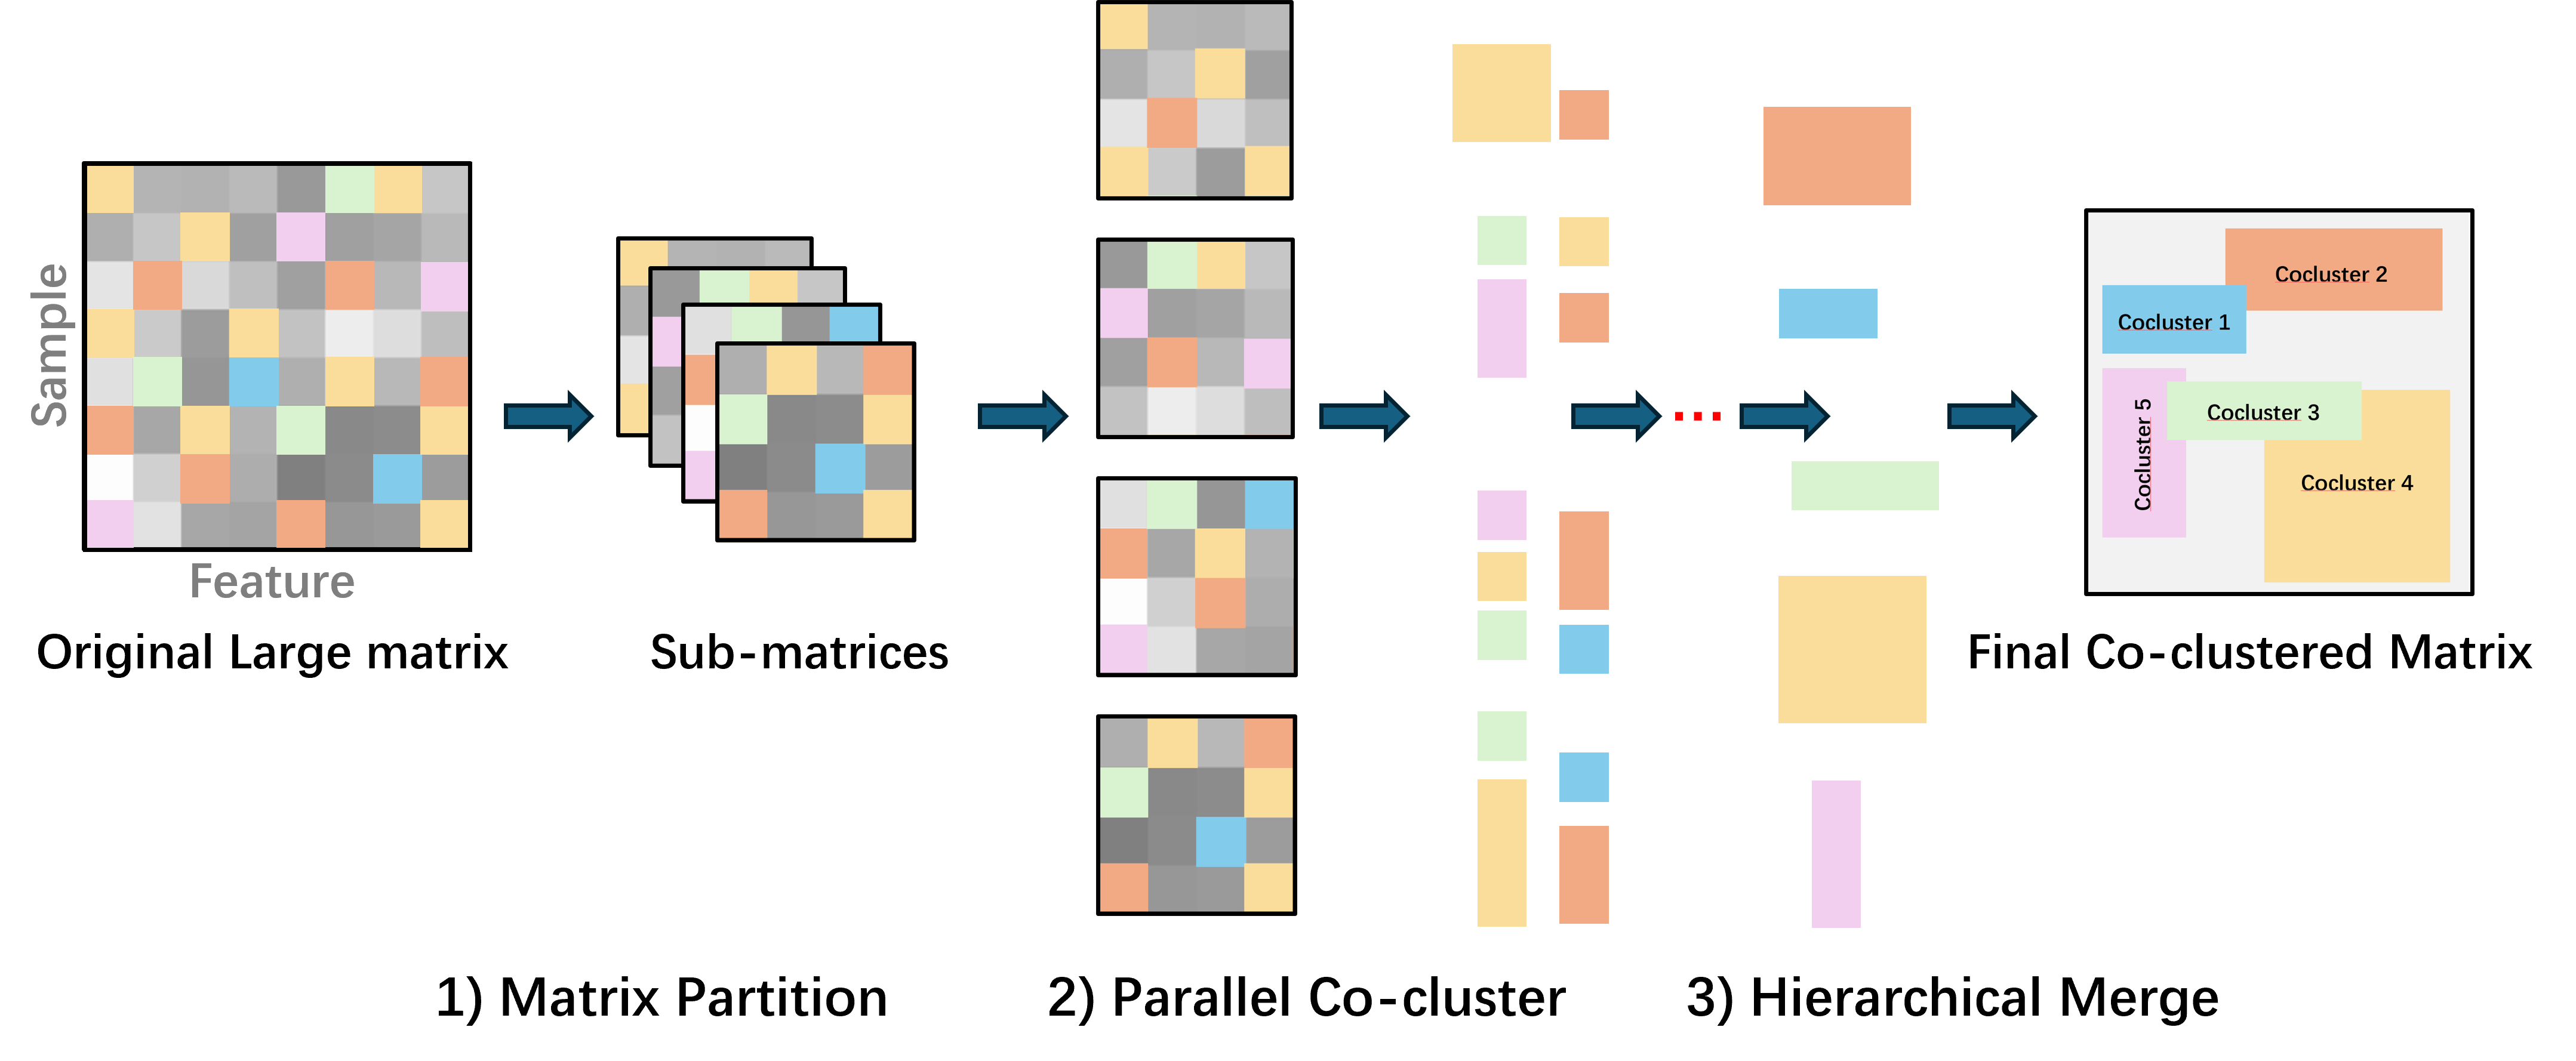
\includegraphics[width=0.8\linewidth]{workflow.png}
    \caption{Workflow of our proposed scalable co-clustering method for large matrices.}
    \label{fig:workflow}
\end{figure*}
This paper presents a novel and scalable co-cluster method specifically designed for large matrices, as shown in \Cref{fig:workflow}. This method applies a probabilistic model-based optimal partitioning algorithm, which not only predicts the ideal number and sequence of partitions for maximizing computational efficiency but also ensures the effectiveness of the co-clustering process.

Our method involves partitioning large matrices into smaller, manageable submatrices. This strategic partitioning is meticulously guided by our algorithm to facilitate parallel processing. By transforming the computationally intensive task of co-clustering a large matrix into smaller, parallel tasks, our approach significantly reduces computational overhead and enhances scalability.

Following the partitioning, each submatrix undergoes a co-clustering process. This is implemented via the application of Singular Value Decomposition (SVD) and $k$-means clustering on the resulting singular vectors. This pivotal step ensures the adaptability of our method, allowing our algorithm to tailor its approach to the unique characteristics of each submatrix, thus optimizing clustering results.

Furthermore, our method integrates a novel hierarchical merging strategy that combines the co-clustering results from all submatrices. This integration provides more fine-grained insight into each submatrix and enhances the overall accuracy and reliability of the co-clustering results. Our method, validated and optimized through a comprehensive process, showed efficiency in handling large-scale datasets that were never reached before.  
 

\subsection{Large Matrix Partitioning}
% Description of the matrix partitioning process and criteria for partitioning.
The primary challenge in co-clustering large matrices is the risk of losing meaningful co-cluster relationships when the matrix is partitioned into smaller submatrices. To address this, we introduce an optimal partitioning algorithm underpinned by a probabilistic model. This model is meticulously designed to navigate the complexities of partitioning, ensuring that the integrity of co-clusters is maintained even as the matrix is divided. The objective of this algorithm is twofold: to determine the optimal partitioning strategy that minimizes the risk of fragmenting significant co-clusters and to define the appropriate number of repartitioning iterations needed to achieve a desired success rate of co-cluster identification.

\subsubsection{Partitioning and Repartitioning Strategy based on the Probabilistic Model}
Our probabilistic model serves as the cornerstone of the partitioning algorithm. It evaluates potential partitioning schemes based on their ability to preserve meaningful co-cluster structures within smaller submatrices. The model operates under the premise that each atom-co-cluster (the smallest identifiable co-cluster within a submatrix) can be identified with a probability $p$. This probabilistic model allows us to estimate the likelihood of successfully identifying all relevant co-clusters across the partitioned submatrices.

In the scenario where the matrix $A$ is partitioned into $m \times n$ blocks, each block has size $\phi_i \times \psi_j$, that is, $M=\sum_{i=1}^m \phi_i$ and $N=\sum_{j=1}^n \psi_j$, the joint probability of $M_{(i,j)}^{(k)}$ and $N_{(i,j)}^{(k)}$ are
\begin{align*}
    P(M_{(i,j)}^{(k)} & < T_m, N_{(i,j)}^{(k)} < T_n)                               \\ & = \sum_{\alpha=1}^{T_m-1} \sum_{\beta=1}^{T_n-1} P(M_{(i,j)}^{(k)} = \alpha) P(N_{(i,j)}^{(k)} = \beta) \\
    % pq[x_, y_] := Sum[p[a] * q[b], {a, 1, x-1}, {b, 1, y-1}]
                      & \le \exp[-2 (s_i^{(k)})^2 \phi_i + -2 (t_j^{(k)})^2 \psi_j]
\end{align*}
where $s_i^{(k)}$ and $t_j^{(k)}$ are the minimum row and column sizes of co-cluster $C_k$ in block $B_{(i,j)}$, the size of the co-cluster $C_k$ is $M^{(k)} \times N^{(k)}$, and $M^{(k)}$ and $N^{(k)}$ are the row and column sizes of co-cluster $C_k$, respectively. 

% the size of co-cluster Ck∈RM(k)×N(k)C_k \in \mathbb{R}^{M^{(k)} \times N^{(k)}} that falls into block B(i,j)B_{(i,j)} is M(k)(i,j)×N(k)(i,j)M_{(i,j)}^{(k)} \times N_{(i,j)}^{(k)};

Thus, the probability of identifying all co-clusters is given by

\begin{align}
    P(\omega_k) & \le \exp \left\{ -2 [\phi m (s^{(k)})^2 + \psi n (t^{(k)})^2] \right\},
\end{align}
and
\begin{align}
    P & = 1 - P(\omega_k)^{T_p}                                                                                                       \\
      & \ge 1 - \exp \left\{ -2 T_p [\phi m (s^{(k)})^2 + \psi n (t^{(k)})^2] \right\} \label{eq:prob_of_identifying_all_co_clusters}
\end{align}
where $P(\omega_k)$ is the probability of the failure of identifying co-cluster $C_k$, $T_p$ is the number of sampling times, $\phi$ and $\psi$ are the row and column block sizes, and $s^{(k)}$ and $t^{(k)}$ are the minimum row and column sizes of co-cluster $C_k$.


\Cref{eq:prob_of_identifying_all_co_clusters} is central to our algorithm for partitioning large matrices for co-clustering, providing a probabilistic model that informs and optimizes our partitioning strategy to preserve co-cluster integrity. It mathematically quantifies the likelihood of identifying all relevant co-clusters within partitioned blocks, guiding us to mitigate risks associated with partitioning that might fragment vital co-cluster relationships.

Based on \Cref{eq:prob_of_identifying_all_co_clusters}, we can establish a constraint between the repartitioning time $Tr$ and the partition solution $Part$, ensuring that the partitioning strategy adheres to a predetermined tolerance success rate, thereby minimizing the risk of co-cluster fragmentation. The constraints are discussed in appendix due to space limitations.

\subsubsection{Optimization and Computational Efficiency}
Optimizing the partitioning process for computational efficiency is paramount in both academic and industrial applications, where running time often serves as the primary bottleneck. Thanks to the flexible framework established by our probabilistic model and the constraints derived in Theorem 1, our optimization strategy can be tailored to address the most critical needs of a given context. In this case, we focus on minimizing the running time without compromising the integrity and success rate of co-cluster identification.
%TODO check the theorem number

Our approach to optimization leverages the probabilistic model to assess various partitioning configurations, balancing the trade-off between computational resource allocation and the need to adhere to theoretical success thresholds. By systematically evaluating the impact of different partitioning schemes on running time, we can identify strategies that not only meet our co-clustering success criteria but also optimize the use of computational resources.

To ensure that our optimization does not sacrifice the quality of co-cluster identification for the sake of efficiency, we introduce a secondary theorem that outlines the conditions under which optimization can be achieved without compromising the success rate of co-cluster discovery. This theorem provides a mathematical basis for optimizing the partitioning algorithm in a manner that maintains a balance between computational efficiency and the fidelity of co-cluster identification.


Under the constraint of maintaining a predetermined success rate $P$ for co-cluster identification, the optimization of the partitioning algorithm with respect to running time must satisfy the following condition:
\begin{align*}
    T_p = \text{argmin}_{T_p} \{ 
     1 &- \exp \{ -2 T_p [\phi m (s^{(k)})^2 \\
     &+ n (t^{(k)})^2] \} \ge P_{\text{thresh}} \} 
\end{align*}


This condition delineates the parameters within which the partitioning strategy can be optimized for speed without detracting from the algorithm's ability to accurately identify co-clusters. By adhering to this theorem, we ensure that our optimization efforts align with the overarching goal of preserving the integrity and effectiveness of co-cluster discovery. This balance is crucial for developing a partitioning algorithm that is not only fast and efficient but also robust and reliable across various data sets and co-clustering challenges.

\subsection{Co-clustering on Small Submatrices}
% Detailed method for co-clustering within each of the submatrices.

\subsubsection{Atom-co-clustering Algorithm}
Our framework, which encompasses both partitioning and ensembling, offers remarkable flexibility, allowing it to be compatible with a wide range of atom-co-clustering methods. For the sake of making this paper comprehensive and self-contained, we provide an introduction to the atom-co-cluster method herein. The only requirement for an atom-co-clustering method to be compatible with our framework is that it must be able to identify co-clusters under a given criterion with a probability $p$, or more relaxed conditions, has a lower bound estimate of the probability of identifying co-clusters equipped with a validation mechanism.

\subsubsection{Graph-based Spectral Co-clustering Algorithm}

Spectral co-clustering (SCC) stands as one of the most prevalent methods in the realm of co-clustering today\cite{vonluxburg2007TutorialSpectralClustering}, primarily due to its adeptness in unraveling the complexities of high-dimensional data. At its core, this method harnesses the power of spectral clustering principles, focusing on the utilization of a graph's Laplacian matrix eigenvectors for effectively partitioning data into distinct clusters. This approach is exceptionally beneficial for analyzing data that naturally forms a bipartite graph structure, including applications in text-document analysis, social network modeling, and gene expression studies.


\paragraph{Graph Construction in Co-clustering Expanded}

SCC begins with constructing a bipartite graph $G=(U,V,E)$. Here, $U$ and $V$, both as vertex sets, symbolize the sets corresponding to the rows and columns of the data matrix, respectively. The edges $E$ of this graph are assigned weights reflecting the relationships between rows and columns. Consequently, the graph's weighted adjacency matrix $W$ is defined as:

$$ W = \begin{bmatrix} 0 & A \\ A^T & 0 \end{bmatrix}, $$
where $A$ denotes the data matrix, also called adjacency matrix in the graph context.
Through this representation, the challenge of co-clustering is reformulated into a graph partitioning task, aiming to segregate the graph into distinct clusters based on the interrelations between the data matrix's rows and columns.

\paragraph{Laplacian Matrix}

The graph's Laplacian matrix $L$ is computed as $L=D-W$, with $D$ being the graph's degree matrix—a diagonal matrix whose entries equal the sum of the weights of the edges incident to each node. The Laplacian matrix plays a crucial role in identifying the graph's cluster structure. It does so by facilitating the calculation of eigenvectors associated with its smallest positive eigenvalues, which in turn, guide the partitioning of the graph into clusters.

\paragraph{Graph Partitioning and Singular Value Decomposition}
Theorem 4 in \cite{dhillon2001CoclusteringDocumentsWords} states that the eigenvector corresponding to the second smallest eigenvalue of the following eigenvalue problem gives the generalized partition vectors for the graph:

\begin{equation}
    L \mathbf{v} = \lambda D \mathbf{v}
    \label{eq:eigenvalue_problem}
\end{equation}

And according to Section 4 of \cite{dhillon2001CoclusteringDocumentsWords}, the singular value decomposition of the normalized matrix $A_n = D^{-1/2} A D^{-1/2}$
$$A_n = U \Sigma V^T$$
gives the solution to \Cref{eq:eigenvalue_problem}. To be more specific, the singular vectors corresponding to the second largest singular value of $A_n$ is the eigenvector corresponding to the second smallest eigenvalue of \Cref{eq:eigenvalue_problem}.

The above discussion is under the assumption that the graph has only one connected component. In a more general setting, $\mathbf{u_2}, \mathbf{u_3}, \ldots, \mathbf{u_{l+1}}$ and $\mathbf{v_2}, \mathbf{v_3}, \ldots, \mathbf{v_{l+1}}$ reveal the $k$-modal information of the graph, where $\mathbf{u_k}$ and $\mathbf{v_k}$ are the $k$-th left and right singular vectors of $A_n$, respectively.
And for the last step,
$$ Z = \begin{bmatrix} D_1^{-1/2} \hat{U} \\ D_2^{-1/2} \hat{V} \end{bmatrix} $$
is stacked where $\hat{U} = [\mathbf{u_2}; \mathbf{u_3}; \ldots; \mathbf{u_{l+1}}]$ and $\hat{V} = [\mathbf{v_2}; \mathbf{v_3}; \ldots; \mathbf{v_{l+1}}]$. The approximation to the graph partitioning optimization problem is then solved by applying a $k$-means algorithm to the rows of $Z$. More details can be found in \cite{dhillon2001CoclusteringDocumentsWords}.

\subsection{Hierarchical Co-cluster Merging}
% Explanation of how co-clustered results from submatrices are aggregated.

Hierarchical co-cluster merging is a novel approach that combines the results of co-clustering on submatrices to produce a final co-clustered result.
The merging method is designed to enhance the accuracy and robustness of the co-clustering outcome by leveraging the design of the partitioning algorithm. The hierarchical merging process iteratively combines the co-clusters from each submatrix, ensuring that the final co-clustered result is comprehensive and consistent across all submatrices. This iterative merging process is crucial for addressing issues of heterogeneity and model uncertainty, ensuring that the final co-clustering results are reliable and robust.

\subsection{Algorithmic Description}
% Step-by-step algorithmic description of the process in pseudocode.
Our proposed  Optimal Matrix Partition and Hierarchical Co-cluster Merging Method is outlined in Algorithm \ref{alg:method}. The algorithm
is an advanced algorithm designed for efficient co-clustering of large data matrices. The algorithm begins by initializing a block set based on predetermined block sizes. For each co-cluster in the given set, the algorithm calculates specific values $s^{(k)}$ and $t^{(k)}$, which are then used to determine the probability $P(\omega_k)$ of each co-cluster. If this probability falls below a predefined threshold $P_{\text{thresh}}$, the algorithm partitions the data matrix $A$ into blocks $B$ and performs co-clustering on these blocks. This step is crucial for managing large datasets by breaking them down into smaller, more manageable units. After co-clustering, the results from each block are aggregated to form the final co-clustered result $\mathcal{C}$. The algorithm's design allows for a flexible and efficient approach to co-clustering, particularly suited to datasets with high dimensionality and complexity.

\begin{algorithm}[!t]
    \caption{Optimal Matrix Partition and Hierarchical Co-cluster Merging Method}\label{alg:method}
    \begin{algorithmic}[1]
        \REQUIRE{Data matrix $A \in \mathbb{R}^{M \times N}$, Co-cluster set $C = \{C_k\}_{k=1}^K$, Block sizes $\{\phi_i\}_{i=1}^m$, $\{\psi_j\}_{j=1}^n$, Thresholds $T_m$, $T_n$, Sampling times $T_p$, Probability threshold $P_\text{thresh}$;}
        \ENSURE{Co-clustered result $\mathcal{C}$;}
        \STATE Initialize block set $B = \{B_{(i,j)}\}_{i=1}^m,_{j=1}^n$ based on $\phi_i$ and $\psi_j$
        \STATE Calculate $s^{(k)}$ and $t^{(k)}$ for each co-cluster $C_k$
        \FOR{$k=1$ to $K$}
        \STATE Calculate $P(\omega_k)$ for co-cluster $C_k$
        \IF{$P(\omega_k) < P_{thresh}$}
        \STATE Partition matrix $A$ into blocks $B$ and perform co-clustering
        \STATE Aggregate co-clustered results from each block
        \ENDIF
        \ENDFOR
        \RETURN Aggregated co-clustered result $\mathcal{C}$
    \end{algorithmic}
\end{algorithm}
